\documentclass{article}

\usepackage{graphicx}
\usepackage{datetime}
\usepackage[a4paper, margin=1.5in]{geometry}
\usepackage{listings}

\lstset{
  language=SQL,  aboveskip=3mm,  belowskip=3mm,  showstringspaces=false,  columns=flexible,  basicstyle={\small\ttfamily},
  numbers=none,
  breaklines=true,
  breakatwhitespace=true,
  tabsize=3
}

\title{\textbf{Café Webseite}}
\newdateformat{mydate}{\THEDAY\ \monthname[\THEMONTH] \THEYEAR}
\date{\mydate\today}
\begin{document}

\maketitle
\begin{center}

\author{\textbf{Silvan Lendi, Fabio Zahner}}
\end{center}

\newpage
\tableofcontents
\newpage

\section{Excercise 2.2.1}


Im ersten Schritt gilt es den S3 Bucket zu erstellen und die Dateien in den Bucket zu entzippen. Wir hatten bereits Anfangs Berechtigungsprobleme beim Erstellen des Buckets, da wir die gute Idee hatten, die Region auf EU-West-1 zu wechseln.

Die Webseite ist nun über den Link zugreiffbar, allerdings werden die Bilder nicht geladen.

Damit die vollständige Webseite richtig angezeigt wird, und das statische hosting richtig funktioniert, müssen einige Einstellungen des Buckets geändert werden.


\section{Excercise 2.2.2}

\begin{itemize}
	\item Die Blockierung von allen öffentlichen Zugriffen aufheben.
	
	
	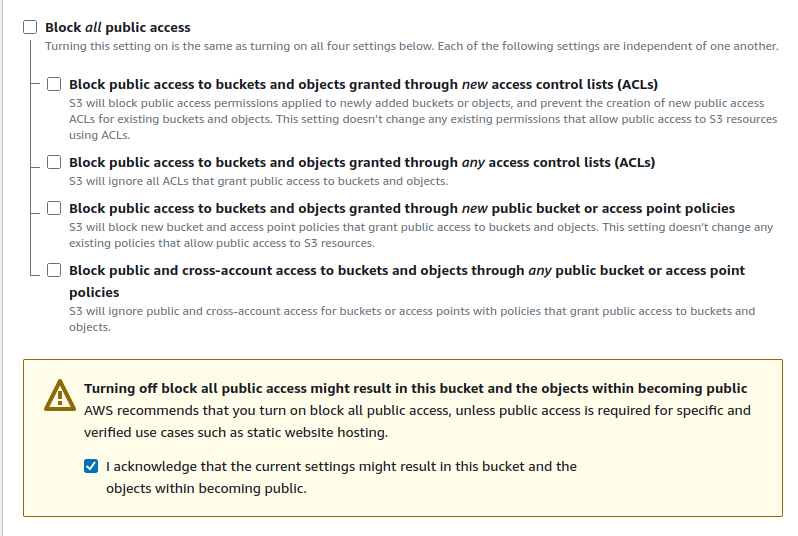
\includegraphics[width=\textwidth]{images/accesslist.png}
	
	\item Statisches Website-Hosting eingeschaltet und Indexdokument gesetzt.
	
	
	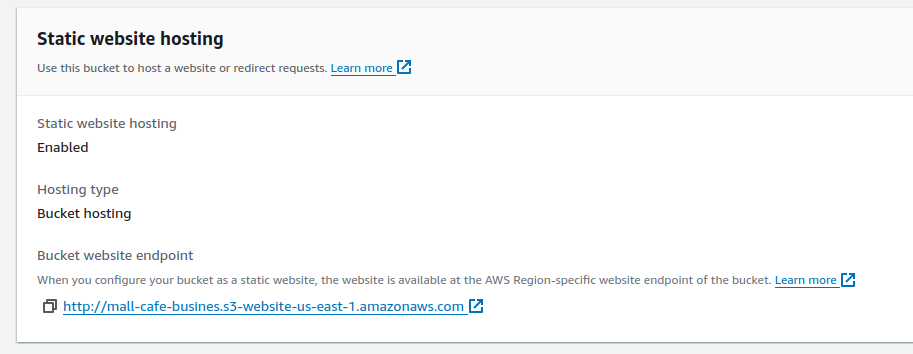
\includegraphics[width=\textwidth]{images/staticwebsitehosting.png}
	\pagebreak
	\item Bucket-Policies gesetzt
	
	
	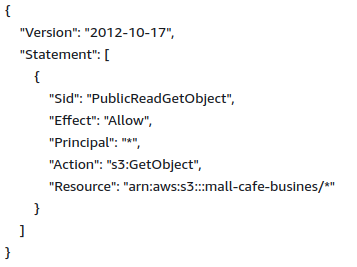
\includegraphics[width=200px]{images/jsonpermission.png}

\end{itemize}


\bigskip



\end{document}
